\documentclass[12pt]{report}
\usepackage[fontsize=13pt]{scrextend}
\usepackage[utf8]{vietnam}
\usepackage[utf8]{inputenc}
\usepackage[english]{babel}
\usepackage{titlesec}
\usepackage{titletoc}
\usepackage{listings}
\usepackage[bookmarks=true]{hyperref}
\usepackage[left=3cm,right=2cm,top=2.5cm,bottom=3cm]{geometry}
\usepackage{graphicx}
\usepackage{hyperref}
\usepackage{tikz}
\usepackage{varwidth}
\usepackage{dirtytalk}
\usepackage{float}
\usepackage{listings}
\usepackage{color}
\usepackage{multirow}
\usepackage{booktabs}
\usepackage[ruled,vlined]{algorithm2e}
\usepackage{chngcntr}
\usepackage{nameref}

%\usepackage[font=bf]{caption}
%\counterwithin{figure}{chapter}

\renewcommand\labelitemi{--}

\setlength{\parskip}{6pt}

\usetikzlibrary{calc}
\setlength{\parindent}{10mm}
\renewcommand{\baselinestretch}{1.3}
\graphicspath{{images/}}

%%% The following lines add Chapter or Appendix in front of the number
\titlecontents{chapter}%
[0pt]%
{\vspace{1ex}}%
{\bfseries Chapter \thecontentslabel\quad}%
{\bfseries}%
{\bfseries\hfill\contentspage}
%%% Initially, for the main part of the document, set the label to "Chapter"
\let\chapappname\chaptername

\definecolor{dkgreen}{rgb}{0,0.6,0}
\definecolor{gray}{rgb}{0.5,0.5,0.5}
\definecolor{mauve}{rgb}{0.58,0,0.82}

% setup code area as listings
\lstset{frame=tb,
  language=Java,
  aboveskip=3mm,
  belowskip=3mm,
  showstringspaces=false,
  columns=flexible,
  basicstyle={\small\ttfamily},
  numbers=left,
  numberstyle=\tiny\color{gray},
  keywordstyle=\color{blue},
  commentstyle=\color{dkgreen},
  stringstyle=\color{mauve},
  breaklines=true,
  breakatwhitespace=true,
  tabsize=3
}

\renewcommand{\lstlistingname}{Source code}

\newenvironment{thuattoan}[1][h]
  {\renewcommand{\algorithmcfname}{Algorithm}
   \begin{algorithm}[#1]
  }{\end{algorithm}}

% hyper setup
\hypersetup{
	bookmarks=true,
	pdftitle={A generative adversarial network for handwritten Japanese characters generation},
	pdfauthor={Phạm Thái Sơn}, % author
	pdfsubject={TeX and LaTeX},
	pdfkeywords={TeX, LaTeX, graphics, images}, % list of keywords
	colorlinks=false,       % false: boxed links; true: colored links
	linkcolor=black,       % color of internal links
	citecolor=black,       % color of links to bibliography
	filecolor=black,        % color of file links
	urlcolor=black,        % color of external links
	linktoc=page,            % only page is linked
}

\begin{document}
\begin{titlepage}
	\center
	\begin{tikzpicture}[overlay,remember picture]
		\draw [line width=3pt,rounded corners=0pt,]
		($ (current page.north west) + (25mm,-25mm) $)
		rectangle
		($ (current page.south east) + (-15mm,25mm) $);
		\draw [line width=1pt,rounded corners=0pt]
		($ (current page.north west) + (26.5mm,-26.5mm) $)
		rectangle
		($ (current page.south east) + (-16.5mm,26.5mm) $);
	\end{tikzpicture}
	
	{\large \bfseries ĐẠI HỌC QUỐC GIA HÀ NỘI\\ TRƯỜNG ĐẠI HỌC CÔNG NGHỆ}\\[1cm]
	\includegraphics[width=0.2\linewidth]{uet}\\[1cm]
	{\Large  \bfseries Phạm Thái Sơn}\\[1.5cm]
	{ \LARGE \bfseries A GENERATIVE ADVERSARIAL NETWORK  FOR HANDWRITTEN JAPANESE CHARACTERS GENERATION}\\[0.5cm]
	\hfill\\[1.5cm]
	{\large \bfseries KHÓA LUẬN TỐT NGHIỆP ĐẠI HỌC HỆ CHÍNH QUY}\\	
	{\large \bfseries Ngành: Khoa học máy tính CLC}	
	\hfill\\[3.5cm]	
	{\large \bfseries HÀ NỘI - 2021}\\	
	\vfill
\end{titlepage}
	
%-----SECONDARY TITLE PAGE-----%	
\begin{titlepage}
	\center
	\begin{tikzpicture}[overlay,remember picture]
		\draw [line width=3pt,rounded corners=0pt,]
		($ (current page.north west) + (25mm,-25mm) $)
		rectangle
		($ (current page.south east) + (-15mm,25mm) $);
		\draw [line width=1pt,rounded corners=0pt]
		($ (current page.north west) + (26.5mm,-26.5mm) $)
		rectangle
		($ (current page.south east) + (-16.5mm,26.5mm) $);
	\end{tikzpicture}
	
	{\large \bfseries ĐẠI HỌC QUỐC GIA HÀ NỘI\\ TRƯỜNG ĐẠI HỌC CÔNG NGHỆ}\\[2cm]

	{\Large  \bfseries Phạm Thái Sơn}\\[2cm]		
	{\LARGE \bfseries A GENERATIVE ADVERSARIAL NETWORK FOR HANDWRITTEN JAPANESE CHARACTERS GENERATION}\\[0.5cm]
	\hfill\\[1.5cm]
	{\large \bfseries KHÓA LUẬN TỐT NGHIỆP ĐẠI HỌC HỆ CHÍNH QUY}\\	
	{\large \bfseries Ngành: Khoa học máy tính CLC}
	\hfill\\[2cm]
	\begin{flushleft}
		{\large \bfseries Cán bộ hướng dẫn: TS. Đào Thành Chung}\\	
	\end{flushleft}
	\hfill\\[3cm]		
	{\large \bfseries HÀ NỘI - 2021}\\		
	\vfill		
\end{titlepage}

%-----TERTIARY TITLE PAGE-----%	
\begin{titlepage}
	\center
	\begin{tikzpicture}[overlay,remember picture]
	\draw [line width=3pt,rounded corners=0pt,]
	($ (current page.north west) + (25mm,-25mm) $)
	rectangle
	($ (current page.south east) + (-15mm,25mm) $);
	\draw [line width=1pt,rounded corners=0pt]
	($ (current page.north west) + (26.5mm,-26.5mm) $)
	rectangle
	($ (current page.south east) + (-16.5mm,26.5mm) $);
	\end{tikzpicture}
	
	{\large \bfseries VIETNAM NATIONAL UNIVERSITY, HA NOI\\ UNIVERSITY OF ENGINEERING AND TECHNOLOGY}\\[2cm]
	
	{\Large  \bfseries Pham Thai Son}\\[2cm]		
	{ \LARGE \bfseries A GENERATIVE ADVERSARIAL NETWORK FOR HANDWRITTEN JAPANESE CHARACTERS GENERATION}\\[0.5cm]
	\hfill\\[1.5cm]
	{\large \bfseries BACHELOR'S THESIS}\\	
	{\large \bfseries Major: Computer Science}
	\hfill\\[3cm]
	\begin{flushleft}
		{\large \bfseries Supervisor: Dr. Dao Thanh Chung}\\	
	\end{flushleft}
	\hfill\\[3cm]		
	{\large \bfseries HANOI - 2021}\\		
	\vfill		
\end{titlepage}


\newpage
\pagenumbering{roman}
\begin{center}
	\textbf{\large DECLARATION OF AUTHORSHIP}
\end{center}

% \addtocontents{toc}{\vspace{1em}}  % Add a gap in the Contents, for aesthetics

\emph{
\say{I hereby declare that the work contained in this thesis is of my own and has not been previously submitted for a degree or diploma at this or any other higher education institution. To the best of my knowledge and belief, the thesis contains no materials previously published or written by another person except where due reference or acknowledgement is made.}
}
\bigskip
\begin{flushright}
	\begin{varwidth}{\linewidth}\centering
		Student\\[2cm]
		Pham Thai Son
	\end{varwidth}
\end{flushright}
\clearpage  % Declaration ended, now start a new page

%% ----------------------------------------------------------------
% Approval
\pagenumbering{roman}
\begin{center}
	\textbf{\large SUPERVISOR'S APPROVAL}
\end{center}

%\addtocontents{toc}{\vspace{1em}}  % Add a gap in the Contents, for aesthetics

\emph{
\say{I hereby approve that the thesis in its current form is ready for committee examination as a requirement for the Bachelor of Computer Science degree at the University of Engineering and Technology.}
}
\bigskip
\bigskip
\bigskip

Signature .............................................................................

\clearpage  % Declaration ended, now start a new page

%-----THANKS-----%
\newpage
\pagenumbering{roman}
\begin{center}
	\textbf{\large ACKNOWLEDGEMENTS}
\end{center}
I would like to express my sincerest gratitude to my my advisors, Dr. Nguyen Thi Ngoc Diep and Dr. Dao Thanh Chung, who have provided me with guidance and assistance during the making of this thesis. Their valuable feedback and insights have help me find the right direction to complete this research. Without their guidance, this thesis would not have been possible.

Additionally, I would also like to thank all the members of the Faculty of Information and Technology for providing me with valuable knowledge throughout my college years. I would also like to extend my gratitude to my lab mates and classmates from K62-CACLC3.

Last but not least, I would like to acknowledge the supports from my friends and family throughout my years of study at UET.
	
%-----ABSTRACT-----%
\newpage
\begin{center}
	\textbf{\large TÓM TẮT}
\end{center}
Ngày nay, trong thời đại công nghệ thông tin, nhu cầu số hóa các dữ liệu giấy tờ ngày càng trở nên cần thiết. Các dữ liệu này bao gồm giấy tờ, tài liệu, các thông tin trên các dữ liệu này thường được viết bằng tay. Phương pháp phổ biến nhất hiện nay để số hóa các dữ liệu này
là sử dụng Optical Character Recognition để nhận diện mặt chữ cái viết tay để chuyển chữ thành dạng trên máy tính. Để làm được điều này, cần huấn luyện một mạng học sâu nhận diện chữ cái viết tay, do vậy, một lượng dữ liệu chữ viết tay lớn là cần thiết để tăng độ chính xác của mô hình. Đối với các bảng chữ cái hình họa như tiếng Nhật, tiếng Trung, việc thu thập dữ liệu chữ viết tay là một điều rất khó để làm so với các bảng chữ latin như tiếng Anh hay tiếng Việt. Lý do là vì bảng chữ cái của Nhật có hơn 50,000 ký tự Kanji khác nhau, trong đó có hơn 2,000 từ là kanji thông dụng được sử dụng trong cuộc sống hàng ngày.

Chính vì thế, một phương pháp để tự động sinh ra các dữ liệu này từ những dữ liệu đã có là điều cần thiết. Trong bài khóa luận này, em xin được đề xuất một phương pháp sử dụng mạng học sâu Generative Adversarial Network để tự động sinh dữ liệu chữ viết tay Nhật Bản từ dữ liệu chữ font đã sẵn có.

%-----ABSTRACT (ENGLISH)-----%
\newpage
\begin{center}
	\textbf{\large ABSTRACT}
\end{center}
Kanji is a very important aspect in Japanese literature and everyday life. In the digital age, the needs to digitized handwritten documents is also increasingly becoming important. Optical Character Recognition (OCR) is widely used for this purpose. But one of the hardest problem to tackle is perhaps identifying written kanji, since there is such a large amount of characters in the kanji writing system, OCR model can fail when met with an unfamiliar kanji given the shortage of quantity and variety of data samples. Thus this research project seeks to expand upon the existing dataset by leveraging the generative capability of Generative Adversarial Networks to synthesize new samples from existing data, using a variety of generative techniques that has been proven to produce highly authentic results. Another goal is to provide a pre-trained model capable of synthesizing data samples for new data samples.
The currently available ETL Japanese handwritten dataset \cite{etl} currently has roughly 200 samples for over 2000 kanji character, with this project, a more variety of samples and new data can be added.

%-----TOC-----%
\newpage
\tableofcontents

\newpage
\addcontentsline{toc}{chapter}{\listtablename}
\listoftables

\newpage
\addcontentsline{toc}{chapter}{List of abbreviations}
\begin{flushleft}
\bfseries{\Huge{List of abbreviations}}
\end{flushleft}
\begin{table}[h]
	\centering
	\begin{tabular}{lll}
		\textbf{GAN}  & Generative Adversarial Network\\[0.3cm]
		\textbf{OCR}  & Optical Characters Recognition              \\[0.3cm]
		\textbf{VAE} & Variation autoencoder \\[0.3cm]
		\textbf{MUNIT} & Multimodal Unsupervised Image-to-Image Translation \\[0.3cm]	
		\textbf{KL loss} & Kulback-Leibler divergence \\[0.3cm]
		\textbf{cGAN} & Conditional Generative Adversarial Network \\[0.3cm]
		\textbf{cVAE} & Conditional Variational Autoencoder \\[0.3cm]
	\end{tabular}
\end{table}

\newpage
\addcontentsline{toc}{chapter}{\listfigurename}
\listoffigures

%-----MAIN-----%
\newpage
\pagenumbering{arabic}
\setcounter{page}{1}
\chapter{Introduction}
\label{chap:intro}

\section{Motivation}
The availability of a large sample database is very important to design high accuracy
classifiers for handwritten characters recognition. Though, for such a database to be manually collected either from human writers or practical documents is expensive, particularly for large characters set, for example, the Japanese Kanji. To
collect a sufficient quantity is a time-consuming and expensive task, much more so
for a large characters set such as the Japanese Kanji writing system with over 50,000
characters in total and more than 2,000 commonly used characters. Kanji are
commonly used in every aspect of Japanese’s daily life such as documents writing,
especially handwritten Kanji.
Japanese Kanji writing system has a complex structure and rules of writing that
requires years of practice and memorization. Such skills for a long time were
essential in education, employment or living in Japan. However, in the digital age
this might no longer be the case with the prevalent of electronic devices such as
phones, computers, the needs for writing Kanji are becoming less and less important.
Though, many people in Japan still consider handwriting an art form like calligraphy
or as an artistic expression. The needs for handwritten Kanji however have not
disappeared, as documents are still filled out by hands, or old literature that needs to be preserved, and thus need to be digitized. To digitize such large amounts of data manually would be expensive and time-consuming, that’s
why a high accuracy optical recognition model is a very important in order to
automate this process. Thus, the needs for a sufficient database samples is needed.
One of the hardest problem to tackle is perhaps identifying written kanji, since there
is such a large amount of characters in the kanji writing system, OCR model can fail
when met with an unfamiliar kanji given the shortage of quantity and variety of data
samples. Thus this research project seeks to expand upon the existing dataset by
leveraging the generative capability of Generative Adversarial Networks to
synthesize new samples from existing data, using a variety of generative techniques
that has been proven to produce highly authentic results. Another goal is to provide
a pre-trained model capable of synthesizing data samples for new data samples.
The currently available ETL Japanese handwritten dataset \cite{etl} currently has roughly 200
samples for over 2000 kanji character, with this project, a more variety of samples
and new data can be added.

\section{Research objective}
The goal of this research is to improve upon the existing handwritten Japanese dataset by 
using deep learning generative based method.
The existing ETL dataset has provided sufficient samples for the hiragana and
katakana alphabets with more than 2000 samples for each characters, meanwhile,
only a handful of kanji handwritten samples have been provided, not to mention, not
all samples are handwritten but are actually in font style.
Since Chinese characters and the Kanji writing system are so similar, I decided to
take a look at both domains of research. Existing generative methods for similar
logographic alphabets have mainly been focusing on generating Chinese calligraphy
rather than handwritten styles, this may be due to the fact that there is already a
widely used handwritten Chinese dataset \cite{casia}, and not a lot of focus has been on
generating handwritten Japanese kanjis in particular, or even Chinese characters. This
research aims to address the lacks of models for generating handwritten Kanji.

\section{Contribution}
In this thesis, we propose a new model that combines approaches from previous works MUNIT\cite{munit} and GANimorph\cite{ganimorph} by using the variational-autoencoder generators from MUNIT and dilated discriminators from GANimorph to diversify the styles and shapes of generated handwritten characters, along with auxiliary losses for preserving the characters structure. We compare our results with image-to-image translation model like CycleGAN\cite{cycle-gan}, as well as with the original MUNIT\cite{munit} model and show that our model can generate a more stable and diverse results.

\section{Thesis organization}
The rest of this thesis will be catagorized as follow \textbf{Chapter \ref{chap:background}} will introduce prerequisites knowledge for our methodology. \textbf{Chapter \ref{chap:methodology}} Outlines our proposed method, implementations as well as go into details of some neccessary theories. \textbf{Chapter \ref{chap:experiments}} Experiments done with CycleGAN and the proposed model, comparision between results of the 2 networks. \textbf{Chapter \ref{chap:conclusion}} final conclusion of the thesis as well as the achieved results, future plans.


\newpage	
\chapter{Background}
\label{chap:background}

\section{Challenges in handwritten text generation}

In contrast to phonological languages like English which only has 26 letters in their alphabets, logographic languages like Japanese have well over 50,000 kanji letters in existent, with over 2,000 commonly used kanjis. These numbers make it much more challenging to produce a personalized font for kanji characters.
Most methods for English character generation utilized the sequential nature of handwritten English text in order to produce realistic results since each character written in English is influenced directly by what’s written in front of it. Thus, in order to capture the realistic nature of the text, generative model like \cite{scrabble-gan} use only as many as 1 style noise to guide the whole generative process since characters are influenced by each other, the whole text need only be in 1 style. Logographic alphabet like Japanese are more difficult to produce realistically handwritten samples since the strokes in logogram writing system are not sequential, they are not influence directly by what character are written before them but rather follows a set of rules and orders which can be more difficult to quantify as a mathematical or logical problem. Handwritten style for characters such as these can also be difficult to produce since each strokes are not always connected directly or followed each other sequentially which poses difficulty when attempting to imitate such style globally.

Early methods like \cite{automatic-calligraphy}, \cite{automatic-handwritten} use the split and merge approach where characters are decomposed into components, then merge back together using some form of synthesize algorithm to produce new samples of writing style, either handwritten or calligraphy. These approaches are limited in that they can only focus on the local representation of the decomposed strokes rather than the whole style of the character, also that logogram characters with complex structure are difficult to be decomposed automatically, and require manual decomposition for certain styles to assure structural integrity such as the cursive script \cite{intel-system}.
Online based methods \cite{online-kanji} \cite{online-kanji-2} are able to produce believable images but doesn’t have the uniform thickness a handwritten character should have and suffer from the same problem of localized representation rather than globally. Obtaining online dataset can also be difficult and much more difficult to process than offline dataset.
GANs approaches like \cite{zi2zi}\cite{handwritten-cgan}\cite{calligan}\cite{scrabble-gan}\cite{gan-writting} incorporate a recognizer network to promote realism in generated images. \cite{gan-writting} focuses more on out of vocabulary word generation rather than character structure. While \cite{scrabble-gan} is implemented with sequential words in mind rather than logographic characters. \cite{zi2zi} requires paired dataset and this can be hard to obtain given how many Kanjis there are, it would be infeasible to ask volunteers to write thousands of characters. \cite{handwritten-cgan} provides an interesting combination of both cGAN \cite{cgan} and cVAE \cite{cvae} but haven’t able to produce tangible results. \cite{calligan} so far is the most in-line with this research problem but still has its reliance on external system \cite{casia} and also requires paired dataset.

\section{Approaches}
For over 20 years, there have been many approaches in generating different style characters, be it latin-based or logographic writing system.
Some leveraged the complex structure of Kanji or Chinese characters by decomposing them into components, defined a set of artistic constraints that belongs to different style and impose them onto newly generated samples. Other approaches decomposed training samples characters into components, synthesize and combining them to generate new samples.

Another kind of approaches utilized online instead of offline handwriting samples, meaning data about written strokes by users can be used such as pen trajectory, writing speed and thickness of stroke portions.

Recently, with the development of GAN paradigm, new approaches can utilize powerful generative capabilities of neural network without having to explicitly define constraints in order to generate believable new samples.

\begin{figure}[h]
	\centering
	\includegraphics[scale=0.7]{hierarch-comp}
	\caption{\textit{Hierarchical representation of character components extraction by \cite{handwritten-font}. a) and b) are two possible ways of character composition}}
	\label{fig:hierarch-comp}
\end{figure}

Xu et al.\cite{automatic-calligraphy} decomposed Chinese characters into hierarchical representation of their
strokes, defined a set of artistic constraints for these family of strokes, by means of
data prediction (interpolation or extrapolation), generate new hierarchical strokes
family that must satisfy the set of constraints. The generation algorithm is based on
analogical reasoning process (ARP), where multiple variations of constructive
elements are extracted from training examples and blended together to form a new
variation of the same strokes that must satisfy some aesthetic constraints learned
from the training examples.
Another work done by Xu et al.\cite{automatic-handwritten} attempts to generate personalized Chinese
handwriting by capturing the characteristic of writers through estimating the
likelihood that a character elements belongs under a writer X’s writing style. This
method also decomposed Chinese characters into hierarchical representation of their
strokes, then defined a set of grammar rules for composing the original character
based on these stroke components. The handwritten characteristics are learned by 2
neural networks, these 2 models learn the confidence and likelihood score that are
needed in order for a character element to belong under a specific handwriting style.
The generation algorithm is an optimized version of the ARP process in the previous
work by the same author, tuned for finding the most suitable permutation for a
writing style.
Lin et al.\cite{handwritten-font} proposed collecting handwritten data from users, extracting the
components from characters, synthesized these components then used a selecting
algorithm to randomly generate new characters.
Liu et al\cite{automatic-personalized} used a similar approach by collecting samples of handwritten characters
or character’s components then randomly select written components or characters
following a probability distribution then combining them to generate new samples.
The problems with focusing only on the parameterization of character components
is that it only focuses on the local representation of strokes rather than the whole
style of a characters thus may lead to inconsistency in the generated image as a whole.

Typography is a type of style transfer problems whereby a designer has to arrange the typeface, layout, spacing, grids of words in order to make them appealing and legible with different style. Artistic calligraphy is an art form exist in Chinese or Japanese culture where by characters are written in different styles to convey expressions by the artists. Usually, each artists calligraphy style is different.

Yang et al.\cite{awesome-typography} approach the typography problem by exploiting the analytics on the
high regularity of the spatial distribution for text effects to guide the synthesis
process
Lian et al.\cite{automatic-morphing} tackle shape morphing characters into different style by template
constructing using character skeleton, strokes, key points and connection triangles
for every Chinese character in the standard Kaiti font library, then breakdown the
strokes of the source and target characters to find correspondence values between
them and the template shape, afterward mesh transform the source to target character
by shape interpolation.
Meanwhile zi2zi \cite{zi2zi} utilized generative adversarial network with category
embedding for one-to-many mapping between a character and its many variation in
style in order to generate new samples, however this requires paired dataset and that
can be hard to come by

Liu et al.\cite{online-kanji} utilized on-line databases of written Kanji characters to generate new styles by combining pen trajectory with shape pattern with 3 modes of writing, connected lines, proportional line or kanji style. Connected line modes connect point from the pen trajectory with uniform thickness, while the proportional mode assumes the thickness from the writing speed, and the kanji mode generates character with brush-like characteristic.
Liu et al.\cite{online-kanji-2} an improved approach to \cite{online-kanji}, this new method can cope with connected strokes, decomposed strokes into 3 parts: start part, end part and bend part then paint each part according to a prototypal shape assigned to it from a calligraphy library.

\begin{figure}[h]
	\centering
	\includegraphics[scale=0.65]{style-transfer}
	\caption{\textit{Image style transfer by CycleGAN. First row is the original picture, rest are the original being translated to the respective styles.}}
	\label{fig:style-transfer}
\end{figure}

Current image style transfer methods can be divided into 2 categories \cite{neural-style}, descriptive neural methods or generative neural methods. Descriptive neural methods transfer the styles by computing the gradients between the source and target image then update pixels in the generated image iteratively. Generative neural methods however, first fine tuning a generative model and generate styled images in a single forward pass. The descriptive methods only works for a single target image which makes it time consuming and harder to capture a complete style of a domain, while the generative methods works faster but produce poorer results.

Most GAN\cite{gan} approaches try to incorporate some kind of content or style losses in order to promote realistic looking images. Many attempts to also separate the style and content for better results at style transferring.
\cite{handwritten-cgan} Combines cGAN \cite{cgan} and cVAE \cite{cvae} into one, cVAE (conditional variational autoencoder) is VAE with one hot encoded label of the character as additional input for the encoder. Both model is trained end-to-end by feeding the sample from the latent space generated by the encoder of cVAE conditioned on the class of the character to the cGAN model when training to utilize the semantic of the character generated.
\cite{calligan} trains a generator conditioned on the style label of a writer and the structure of the desired character – by decomposing the character into sequence of components then encode into a component vector. The discriminator is trained on a ground truth (pixel-wise) loss – ensure the similarity between the generated image and ground truth image, adversarial loss – to ensure the generated image looks realistic, constancy loss – ensure the generated image and the font-rendered-image have similar feature vectors. and a category loss – ensure the generated image retained the style of the writer.
\cite{handwritten-cyclegan} proposes using a DenseNet for the transfer module of CycleGAN instead of ResNet. The transfer module handles extracting feature from a domain, using a DenseNet supposedly improves the flows of information through each block by connecting them directly witch each other.

\begin{figure}[h]
	\centering
	\includegraphics[scale=0.9]{handwritten-cycle-gan-result}
	\caption{\textit{Results of Handwritten CycleGAN \cite{handwritten-cyclegan} trained on the HW252 style from the CASIA dataset \cite{casia}.}}
	\label{fig:handwritten-cycle-gan-result}
\end{figure}

\cite{scrabble-gan}, \cite{gan-writting} uses a text recognition network in addition to a discriminator in the GAN paradigm to promotes realistic and readable handwriting styles. In \cite{scrabble-gan}, the generator is a concatenation of multiple convolutional class conditional generators with overlapping receptive fields to simulate influence of characters next to each other in the same word.
Uses a noise vector to control the style generated, the discriminator has to also accounts for the output style of the generated image when discriminating between the fake and real images.
\cite{gan-writting} incorporates style and textual content from 2 learning branches to feed to a generator. Style and content are learnt independently. The content network outputs textual content feature at 2 different levels, low-level feature encodes the different characters that form a word along with their spatial position within the input string. The network is constrained on an alphabet of allowed characters and maximum character length a word can have. This encoding allows the network to produce out of vocabulary (never seen before) words. The other level is global string encoding that concatenate all character embedding into a large one dimensional tensor that will then be injected into the generator.
Has a style loss to control similarity to the style of the input image – the network has a style classifier trained on the real input dataset, a content loss to control the integrity of the input textual content.
\cite{adversarial-gen} uses bidirectional LSTM recurrent layers \cite{lstm} to get an embedding of sequence of the word to be rendered as additional input to the network. The author also added an auxiliary text recognition network to encourage the generator to produced readable images. In order to reconcile the losses between the discriminator and recognizer network, the model also has an affine transformation layer in order to balance the 2 losses before propagating it back to the generator.
\cite{hw-gan} presents a GAN architecture for synthesizing handwritten digital ink text, uses a Path Signature Feature extractor follow by a CNN-LSTM classifier which act as the discriminator in the GAN paradigm.

Since deep learning models offer automation and adaptability to new data, we decided to use the GAN paradigm to approach this problem.

\begin{figure}[h]
	\centering
	\includegraphics[scale=0.8]{scrabble-gan}
	\caption{\textit{Model overview of ScrabbleGAN \cite{scrabble-gan} for latin-based alphabets. The receptive fields are overlapped to simulate influence between characters in a word.}}
	\label{fig:scrabble-gan}
\end{figure}

\section{GAN paradigms}

\begin{figure}[h]
	\centering
	\includegraphics[scale=0.6]{gan-diagram}
	\caption{\textit{High-level diagram of how Generative adversarial network \cite{gan} works. The generator learns from real data input to generate fake samples, the disrciminator evaluates these samples and backpropagate the evaluation score to the generator. This process repeats until both networks reach an equilibrium.}}
	\label{fig:gan-diagram}
\end{figure}

Generative adversarial Network (GAN) is a generative model architecture that was proposed in 2014 by Ian Goodfellow et al.\cite{gan} that works on principles of a zero-sum game between a generator and a discriminator. This architecture has proven to be powerful and effective that has achieved stunning results in several computer vision tasks like inpainting \cite{image-completion}, image-to-image translation \cite{cycle-gan} or in other domains such as speech synthesis \cite{audio-gan} and cross-language translation \cite{nlp}.
GAN consists of 2 networks: Generator (G) and Discriminator (D). Generator generates images by compressing data into latent space and decodes them back to images – done by using encoders and decoders. G will generates new data instances while D evaluates them for authenticity. The Discriminator ‘judges’ the result of Generator -  i.e. the Discriminator decides whether each instance of data that it reviews belongs to the actual training dataset or not - and feed the error back to the Generator. In essence, D learns to determine whether a sample is from a domain data distributions. To quote an example from the original GAN paper \cite{gan}:

\say{The generative model can be thought of as analogous to a team of counterfeiters,trying  to  produce  fake  currency  and  use  it  without  detection,  while  the  discriminative  model  is analogous to the police, trying to detect the counterfeit currency. Competition in this game drives both teams to improve their methods until the counterfeits are indistiguishable from the genuine articles.}

Thus, they are competing each other in a zero-sum game.

Take an example, where we try to generate animals pictures. The Generator generates new images and passes it to the Discriminator, hoping to “trick” the Discriminator in thinking that the new data is real. The Discriminator tries to identify the incoming data from the Generator as fake.
Here are the steps a GAN takes:
\begin{itemize}
	\item First, D learns from real samples from the animals image domain to know how an animal image should look like.
	\item We input some noise into G to generate fake samples.
	\item D evaluates the fake samples to determine whether they belong in the real data (animals) domain. This outputs some probabilities. 
	\item Advesarial losses are calculated, these are propagated back to G, weights of G are then updated.
	\item Repeats until both networks reach an equilibrium of G is able to generate samples that are indistinguishable from the real domains.
\end{itemize}

The Generator is in a feedback loop with the Discriminator. Another thing to point out is that advesarial loss is calculated based on how well D can evaluate the fake samples. When the model converges means that D can't tell that the samples are fake, this however does not indicate whether or not they objectively look like real samples. Thus, the results of GAN trainings should be decided by human examinations.

\[E_x[log(D(x))] + E_z[log(1 - D(G(z)))]\]

Above is the adversarial loss equation in the original GAN paper, where $x$ is a real data instance, $z$ is input for G, $D(x)$ is D's estimated probability for whether $x$ is real, $G(z)$ is fake sample generated by G, $E_x$ is the expected value over all real data instances, $E_z$ is the expected value over all inputs to G, thus will be the expected value over all the generated results as well. In this expression, G tries to reduce the probability that its outputs are detected as fake, so $E_z[log(1-D(G(z)))]$ will be minimized by G since it can't affect the left side of the equation. And vice versa, D tries to maximize the equation.

\section{CycleGAN for unpaired image style transfer and its limitations}

Even though GAN models such as zi2zi \cite{zi2zi} is able to synthesize convincing characters, its requirements for a paired dataset can be expensive and time consuming to fulfill as stated in \textbf{Chapter \ref{chap:intro}}. Thus, we want our method to not rely on paired dataset. 

[example of paired dataset]

In order to tackle the problem of lacking paired dataset, one of the popular model for unpaired image-to-image translation problem is CycleGAN \cite{cycle-gan}. CycleGAN is a multi-purpose Generative Advesarial Network using cycle consistency loss and aversarial loss to give the model a multi-purpose procedure. In our case, we can use the model for collection style transfer.

One of the distinct aspects about CycleGAN\cite{cycle-gan} from other unpaired image-to-image translation models is its cyclic training procedure, wherein 2 pairs of Generator - Discriminator are trained, one for each domain. These 2 pairs learn the mapping functions from one to the other by using a regularize loss function to ensure a regularized latent space between each domains. This training is thus cycle-consistence, meaning a translated image should be able to revert back to its original domain using the mapping function of the corresponding domain, this is enforced by a cycle-consistency loss. This procedure supposedly regularizes the 2 distributions in a large enough dataset wherein an irregularized distribution could cause a set of inputs $x_i$$\in$$X$ to be mapped to any possible permutations of $y_i$$\in$$Y$ instead of the desired output.

[image of cycle consistency training]

However, CycleGAN is limited in its mapping capabilities in that it can only map 1:1 the distribution of 2 domains. Meaning, for one input image there can be only one corresponding image the model can output. This is due to the static input for CycleGAN which is different from conventional GANs that requires a noise vector as input. Whereas CycleGAN takes as input an image from the source domain in the hope that with a large and complex dataset, the input images can serve in place of a noise vector. This effectively eliminates any variables from the data distributions and instead relies on dataset complexity, thus leads to a lacking in variety of the generated results. However, even when equipped with additional noise vector, the CycleGAN cannot generate diversified results as documented in \cite{augmented-cyclegan} 

In order to address the lack of diversity in results of CycleGAN, there has been a number of proposed methods built from the same framework \cite{munit}\cite{bicycle-gan}\cite{disco-gan}\cite{bayesian-cyclegan}. MUNIT\cite{munit} suggests using 2 variational autoencoders (VAE) as generators, each VAE consists of 3 networks - 2 encoders, 1 decoder. One encoder learns to map the image contents to its latent space, the other do the same for images styles. The encoded content and style act as inputs to the decoder. The decoder tries to reconstruct the image based on the 2 inputs. This basically solves the problem of not having any noise in the input as the style vector can act as noise, thus we can have more diversity in the generated results. This architecture is in line with what we are trying to do.

\begin{figure}[h]
	\centering
	\includegraphics[scale=0.2]{street-munit}
	\caption{\textit{One-to-many mapping by MUNIT\cite{munit}}}
	\label{fig:street-munit}
\end{figure}

Another problem of CycleGAN is that it's really hard to change the shape information of a picture. This means that with a translated image, while the style maybe different, the character shape symmetry will remain the same.

\begin{figure}[h]
	\centering
	\includegraphics[scale=0.9]{cycle-gan-result-2}
	\caption{\textit{Lack of shape deformations in CycleGAN results. Left most column is the source image, there are many source images that are similar and each one differs only slightly, other columns are translated images of similar source pictures.}}
	\label{fig:cycle-gan-result-2}
\end{figure}

\begin{figure}[h]
	\centering
	\includegraphics[scale=1]{kanji-example}
	\caption{\textit{Characters generated by CycleGAN. We experimented by augmenting the training data, the results don't yield significant shape deformation.}}
	\label{fig:kanji-example}
\end{figure}


This is due to the patch-based mechanism of CycleGAN's discriminator. Each patch of the generated image is evaluated by the discriminator thus leading it to unable to learn the whole context of the image, effectively preventing the generator from outputting any image that strays too far from the original source \cite{ganimorph}.

\cite{ganimorph} proposed using dilated convolution for the discriminator to improve the shape deformation capabilitiy of CycleGAN. The dilated discriminator can learn the context of the image and thus can evaluate the entire image as a whole. 

For these reasons, we propose combining both of these approaches by MUNIT\cite{munit} which utilizes variational autoencoders for image generation and GANimorph\cite{ganimorph} for discrimination by segmentation to make our KanjiGAN model, with our own auxiliary loss and data augmentation module to diversify and stabilize generated results for the problem of generating handwritten Japanese characters.

\section{Latent space and Variational autoencoder - VAE}
\subsection{Latent space}
Latent representation is a low-dimensional representation  – compressed data - of object in higher dimension. Latent space is the space for latent representation. For example, a feature in 6 dimensional space can be represented as a 2D feature vector through encoding. This vector is the latent representation of that feature in a 2D latent space.
Latent representation usually only holds important features of data –  E.g: a table has 4 legs,… - Similar features will be closer together in the latent space.
\begin{figure}[h]
	\centering
	\includegraphics[scale=1]{latent-space}
	\caption{\textit{Similar shapes are close points in the latent space}}
	\label{fig:latent-space}
\end{figure}

\subsection{Variational autoencoder and distribution matching}
An autoencoder consist of 2 neural network: the encoder and the decoder.
The encoder is a neural net that encodes the input datapoint $x$ into a representation $z$ in the latent space. The encoder learns an efficient compression of the data into lower-dimensional space.
The decoder is another neural net that decodes $z$ into a probability representation of what the original datapoint $x$ (in the original dimension) might look like.
This is how a classical autoencoder works, with the encoder decoder pairs learn a mapping between original data and points in the latent space.

\begin{figure}[h]
	\centering
	\includegraphics[scale=0.7]{autoencoder-architecture}
	\caption{\textit{Classical autoencoder architecture \cite{autoencoder}}}
	\label{fig:autoencoder-architecture}
\end{figure}

A problem with the classical model is without regularisation of the latent space, autoencoders can easily overfit for the training data. That is, 2 close points in the latent space can only be mapped to a single output that the autoencoder has seen in the training data.

[example of irregularized latent space]

Variational autoencoders (VAEs) tackle these problems by encoding the data into distribution in the latent space as well as adding regularization terms (otherwise known as constraints) to enforce a regularized latent space. An effect of regularizing and distribution encoding is a gradient of the generative process where a point sampled from between two close distribution can have characteristics of both distributions. Whereas a irregularised latent space will have scattered mapping distribution of data. The regularization term is express as the Kulback-Leibler divergence (KL loss) \cite{kl-divergence} between the encoded distribution space and the regularized distribution - the expected distribution, which can be Gaussian or any other distributions. 

\begin{figure}[h]
	\centering
	\includegraphics[scale=0.9]{distribution-space}
	\caption{\textit{An effect of regularizing and distribution encoding is a gradient of the generative process where a point sampled from between two close distribution can have characteristics of both distributions.}}
	\label{fig:distribution-space}
\end{figure}

Intuitively, this KL loss denotes the distance between 2 distributions - the encoded latent space and the expected latent space - which has the effect of encouraging the 2 distributions to match each others during training, this is called \textbf{distributions matching}. In our method from \textbf{Chapter ref{chap:methodology}}, this effect can be implicitly learned without KL loss.

\chapter{Methodology}
\label{chap:methodology}

\section{KanjiGAN}

We proposed combining both MUNIT and \cite{ganimorph} approaches by using the generators architecture of MUNIT and discriminator of \cite{ganimorph} while adding a lightly weighted auxiliary structure loss in order to ensure the characters structure.

\subsection{Model architecture}

\begin{figure}[H]
	\centering
	\includegraphics[scale=0.7]{model-overview}
	\caption{\textit{Our model overview. This architecture is borrowed from MUNIT\cite{munit} with some auxiliary components added by us. The 2 VAEs are swapped to learn distribution matching between 2 domains. Where $s_i$ and $c_i$ are respectively style latent code and content latent code of domain $i$. We added an auxiliary HOG loss to preserve the characters structure, as well as a data augmentation module based on \cite{augmentor} that performs elastic distortion on the target domain images, this is to widen the possible samples space for $G_2$.}}
	\label{fig:model-overview}
\end{figure}

Similar to image-to-image translation models \cite{cycle-gan}\cite{bicycle-gan}\cite{disco-gan} and \cite{munit}, our model defines 2 main losses for the generators. That is reconstruction loss and adversarial loss. However, unlike CycleGAN, we don't rely on a cycle-consistency loss as it would impede the shape transformation capability of the generator. Instead to regularize the latent data distribution, our model uses a L1 loss between the encoded content code and the extracted content code of the translated image to enforce distribution matching. 

Our generator architecture is borrowed from the MUNIT model \cite{munit} where each generator is comprised of 2 VAEs that can encode and decode the images content and style features. The encoder $E_i$ and decoder $G_i$ factorizes the domain latent code into a content code $c_i$ and style code $s_i$, the formulation is as followed, with the subscription $i$ = (1, 2) denotes the belonged domain:
\[(c_i, s_i) =  (E_{c_i}(x_i), E_{s_i}(x_i)) = E_i(x_i)\]

To do image-to-image translation, we perform swapping of the encoder-decoder pairs between 2 domains. That is, to translate an image $x_1$$\in$$X_1$ to $X_2$, first, we extract the content latent code $c_1$ of $x_1$ and randomly samples a style latent code $s_2$ from the prior Gaussian distribution $q$($s_2$), then we input these latent codes into $G_2$ to produce the final output image $x_{1\rightarrow2}$ and vice versa for $x_{2\rightarrow1}$. The formulations is as follow:
\[x_{1\rightarrow2} = G_2(c_1, s_2)\]
\[x_{2\rightarrow1} = G_2(c_2, s_1)\]

\subsection{Objective}
Similar to MUNIT\cite{munit}, we use 2 main losses that encourage reconstruction from the generators.
\begin{itemize}
	\item Latent reconstruction: Given content latent code and style latent code encoded during image-to-image translation, we should be able to reconstruct the same latent codes from the output image.
\[L^{c_1}_{recon} = E_{{c_1}\sim p(c_1), s_2 \sim q(s_2)}[||E^c_2(G_2(c_1,s_2)) - c_1||_1]\]
\[L^{s_2}_{recon} = E_{{c_1}\sim p(c_1), s_2 \sim q(s_2)}[||E^s_2(G_2(c_1,s_2)) - s_2||_1]\]
	\item Image reconstruction: Given an image sampled from the training dataset, after encoding and decoding, we should be able to reconstruct the same image.
\[L^{x_1}_{recon} = E_{{x_1}\sim p(x_1)}[||G_1(E^c_1(x_1), E^s_1(x_1)) - x_1||_1]\]
\end{itemize}

We also added a L1 loss between histogram of gradients\cite{hog} of the cross-domain-translated image and the original input image as we found that this helps discourages the generator from over-deforming the original characters shape.

\[L_{HOG} = L_1(HOG(x_1), HOG(x_{1\rightarrow2}))\] 

Adversarial loss is used to encourage indistinguishable generated results from the target domain.

\[L^{x_2}_{GAN} = E_{c_1\sim p(c_1), s_2\sim q(s_2)}[log(1 - D_2(G_2(c_1, s_2)))] + E_{x_2\sim p(x_2)}[log D_2(x_2)]\]

For the discriminator, LSGan objective \cite{ls-gan} is used. Since regular GAN adopts sigmoid cross entropy loss function which can leads to vanishing gradients problems, a least square loss objective will be more effective as it can penalize outlier data so that the generator can generate samples more inline with the real data distribution.

\[L(E_1, E_2, G_1, G_2, D_1, D_2) = L^{x_1}_{GAN} + L^{x_2}_{GAN} + {\lambda}_x(L^{x_1}_{recon} + L^{x_2}_{recon}) \]
\[+ {\lambda}_c(L^{c_1}_{recon} + L^{c_2}_{recon}) + {\lambda}_s(L^{s_1}_{recon} + L^{s_2}_{recon}) + {\lambda}_{HOG}(HOG(x_{1\rightarrow 2}) - HOG(x_1))\]
 
Our total loss is the weighted sum of the reconstruction losses and the adversarial losses as well as our HOG loss. Since we augment the dataset during training, we observe that a lightly weighted HOG loss can help to discourage the generators from over-deforming the characters shape.

Since the encoder decoder pairs are swapped, in order to do distribution matching, the variational autoencoders are expected to match the 2 content latent spaces with each other, while the 2 style latent spaces are matched with a prior Gaussian distribution. Thus, the optimal matching of latent distributions should be:
\[p(c_1) = p(c_2), p(s_1) = q(s_1), p(s_2) = q(s_2)\]
Where $c_i$ is the content latent code, $s_i$ is the style latent code with $i$ = (1, 2). $p$ and $q$ are the encoded distribution latent space and the prior Gaussian distribution, respectively. The above proposition states that the style latent distribution of both domain should match their Gaussian priors and the content latent distributions must be domain-invariant, meaning the content distribution must match. Although no regularization term are explicitly stated, this loss function has the implicit effect of achieving the optimality as stated by MUNIT\cite{munit} in their \textit{Theoretical Analysis}.

Another expected distributions matching is the joint data distribution.
\[p(x_1, x_1\rightarrow2) = p(x_2\rightarrow1, x_2)\]
Where $x_i$ is the source image, $x_{i\rightarrow j}$ is the translation image from domain $i$ to $j$, with $i$, $j$ = (1, 2). In unsupervised training, joint distribution matching is a crucial constraint in many image-to-image translation problem where it enforces the model to learn a matching distributions between both domains when learning the generative process.

\section{Implementations}
\subsection{Generator architecture}
\begin{figure}[h]
	\centering
	\includegraphics[scale=0.8]{gen-architecture}
	\caption{\textit{Generator architecture is from MUNIT\cite{munit}.}}
	\label{fig:gen-architecture}
\end{figure}
The generator architecture is demonstrated in \textbf{Figure \ref{fig:gen-architecture}}. The style encoder includes several strided convolutional layers, followed by a global average pooling and fully connected layer. In the original MUNIT paper\cite{munit}, 64 convolutional layers were used on complex structured images such as scenery, animals, or painting. Since our dataset consists of images with less complicated colors as well as structures, we only used 32 layers for the encoders.

The content encoder downsamples the input with several strided convolutional layers and feed it to several residual blocks \cite{resnet} to further process it, all the convolutional layers are followed by Instance Normalization \cite{instance-norm}. The content encoders also has only 32 convolutional layers.

The decoder reconstruct the image from a pair of content and style codes. The content code is processed with convolutional layers and upsampling, the style code parameters are learned by a Multi layer perceptron (MLP) \cite{mlp} network to generate the applied style. The original MUNIT paper\cite{munit} used a 256 layers MLP while we only used 128.


\subsection{Discriminator architecture}

In the original paper, MUNIT \cite{munit} employs a multi-scale discriminators from \cite{multi-scale-discri} that can evaluate the generated results at 3 different resolution scales that can guide the generators to produce images that are globally consistent with finer details for complicated and high-resolution-required images like scenery, city pictures. However, since our dataset don't posses complex structure nor high resolution, we chose to employ a different discriminator structure that offers a simpler architecture with less overheads of having to deploy 3 different scale discriminator networks and operate on the same idea of global-context-aware discrimination. That is the dilated convolutional discriminator architecture by GANimorph\cite{ganimorph}. 

\begin{figure}[h]
	\centering
	\includegraphics[scale=0.6]{discri-architecture}
	\caption{\textit{Dilated discriminator architecture by GANimorph\cite{ganimorph}. We only use 32 filters for each convolution block instead of 64 in the original paper.}}
	\label{fig:discri-architecture}
\end{figure}

The discriminator architecture is demonstrated in \textbf{Figure \ref{fig:discri-architecture}}. The discriminator is a fully-convolutional segmentation network. A skip connection is used to preserve the network's view of local context.

Previous approaches \cite{cycle-gan}\cite{disco-gan} use patch-based discriminators to evaluate fake samples where patches of the image are evaluated independently and assigned a score, these scores are summed up and is treated as evaluation score for the whole image. This allows for fast convergence on generators since they will only need to focus on generating realistic patches rather than trying to learn global spatial context of the image, thus leads to the fake samples shapes rarely get transformed beyond its original boundary.

\cite{ganimorph} reframed discrimination as a semantic segmentation problem - finding real or fake regions of the image - by using dilated convolution networks for the discriminators. This allows the discriminator to implicitly learn spatial global context as the receptive fields are expanded with each convolution layers, while the skip connection can preserve the local information of its current view, thus, information from further away in the image are taken into account to evaluate whether a region should fit into an image.

\chapter{Experiments}
\label{chap:experiments}
\section{Dataset}

\begin{figure}[h]
	\centering
	\includegraphics[scale=0.9]{data-examples}
	\caption{\textit{Dataset samples of domain A and B}}
	\label{fig:data-examples}
\end{figure}

We tested and trained our model on the existing ETL dataset\cite{etl} which includes both font-styled characters as well as handwritten samples. We used an extractor tool by \cite{etl-extractor} to extract all the Japanese character images from the original dataset.

Our training dataset is separated into 2 domains, a font-styled domain and handwritten domain, denoted A and B respectively. Domain A includes over 5000 samples while domain B has nearly 7000. We selectively chose character images that have only font style samples as our domain A data. While domain B includes a variety of handwritten style samples including images that has background noise like paper texture, white background and some samples from the Lantingkai dataset of CASIA-HWDB\cite{casia} to increase diversity in generated samples.

\section{Experiments}

\subsection{Limitations of CycleGAN}

We trained the original CycleGAN on the prepared dataset with parameters as followed: $lambda_A = 10$, $lambda_B = 10$, $lambda_{idt} = 0.5$. This is the default parameters of the CycleGAN source code as this produce the most balance results for image-to-image translation problems. We trained the network on Colab Pro GPUs for 150 epochs, the first 100 epochs were trained with a learning rate of 0.0002 and linearly decayed to 0 from epoch 101 to 150.

\begin{figure}[h]
	\centering
	\includegraphics[scale=0.8]{150-epochs}
	\caption{\textit{Results of original CycleGAN training for 150 epochs.}}
	\label{fig:150-epochs}
\end{figure}

The results show that the style of domain B is successfully transferred while the content is partially preserved, especially with white background style whereas images with applied noisy background style has lost significantly its content feature. 

We then added another loss which will be called HOG loss, where we calculate Histogram of gradient (HOG) \cite{hog} on the source image, this gives us a vector representation of edge's direction distribution in the original image, this can be considered a description of the character itself. We apply the same process to the translated sample, then calculate the square differences between two vectors, this gives us the HOG loss. The idea is to encourage the generators preserve as much as possible the character features.

[example of the HOG process]

We continued training CycleGAN for an additional 20 epochs with added HOG loss, the parameters are as followed: $lambda_A = 10$, $lambda_B = 10$, $lambda_{idt} = 0.3$, $lambda_{structure} = 0.2$, where $lambda_{structure}$ is weight term for HOG loss.

\begin{figure}[H]
	\centering
	\includegraphics[scale=0.9]{cycle-gan-result}
	\caption{\textit{Results of original CycleGAN training for 170 epochs. One with and one without additional HOG loss.}}
	\label{fig:cycle-gan-result}
\end{figure}

However, since the HOG loss only promotes preservation for the character shape but does not account for the target styles, we found that the generator will deviate from other styles of the target domains in preference of the white background style as it is much easier to reconstruct the character feature in this distribution area, thus leads to a decrease in diversity of generated styles.
 
Since CycleGAN can only do 1:1 mapping, it is hard if not impossible to have diverse results for one input image. Leveraging the fact that ETL dataset has a lot of similar, near identical images of the same characters, we thought it might be possible to have the network map these similar looking pictures to a larger samples space in the target domain. We experimented with this by decreasing $lambda_A$, $lambda_{idt}$ in favor of our $lambda_{structure}$ and $lambda_B$, in the loss function terms. We also augmented samples of domain B by performing elastic distortion on the images. The idea is by decreasing the cycle loss weight of domain A - intuitively, by shifting the generator's attention away from focusing too much on reconstruction of the input image, we can have a more flexible mapping to the target domain space of possible mapping functions while still preserve the original content features by means of enforcing HOG loss. The augmentation was to expand the possible target domain distribution space. However, we didn't notice significant differences with the generated results for similar pictures of same characters.

\begin{figure}[h]
	\centering
	\includegraphics[scale=0.6]{augment-example}
	\caption{\textit{CycleGAN results after doing augmentation and decreasing identity with reconstruction weight terms.}}
	\label{fig:augment-example}
\end{figure}

\subsection{Experiments with MUNIT}

We trained the original MUNIT\cite{munit} network to serve as comparison against our network. We used the same training configurations as that of the edges to handbags experiment in the original paper as this was the most common configurations, with others differ only in miscellaneous configuration fields. The network was trained for 500000 iterations and for the optimizer, we changed the learning rate decay frequency to once every 20000 iterations after the 250000th iteration. We also performed elastic distortion data augmentation on the handwritten domain. The results are shown in \textbf{Figure \ref{fig:munit-results}}.

\begin{figure}[H]
	\centering
	\includegraphics[scale=0.2]{munit-results}
	\caption{\textit{Samples generated by MUNIT\cite{munit}. The source image style is from the ETL dataset. First row is the source image, remaining 2 rows are the generated samples.}}
	\label{fig:munit-results}
\end{figure}

\begin{figure}[H]
	\centering
	\includegraphics[scale=0.2]{munit-results-2}
	\caption{\textit{Samples generated by MUNIT\cite{munit}. The source image style is lantingkai from CASIA-HWDB\cite{casia}. First row is the source image, remaining 2 rows are the generated samples. }}
	\label{fig:munit-results-2}
\end{figure}

We observe that MUNIT was able to generate some convincingly looking samples, especially with the lantingkai font. However, it struggled to maintain the original characters shape in a lot of the style codes with lots of redundant strokes or overly deformed shape as demonstrated in \textbf{Figure \ref{fig:munit-results}}. MUNIT also failed to reconstruct the source content in more complex styles, this is a common problem in all of our experiments.

\subsection{Experiments with KanjiGAN}

Since our model uses VAEs as generators, it is possible to have one-to-many mappings between 2 domains spaces, this is enabled by the distribution matching of style code latent space to a priori, which acts as noise for sampling in the generative process, as well as joint distribution matching of the data latent space.

We trained our model for 150 epochs with learning rate set to 0.0002 for the first 100 epochs then linearly decay to 0 from epoch 101 to 150. The training parameters are as followed: [put params here]. 

\begin{figure}[H]
	\centering
	\includegraphics[scale=0.9]{kanji-gan-results}
	\caption{\textit{Samples generated by our KanjiGAN. First column is the original input, the rest are a variety of styles our model has produced. Though in more complex styles, the model still failed to reconstruct the original content features. The reason could be due to imbalance complexity in the training styles.}}
	\label{fig:kanji-gan-results}
\end{figure}

With the input data now being mapped as distributions in the latent space, with additional style noise, the network should be able to produce differently looking images with a more variety in style. However, we found that the network is only able to reconstruct content of the source image in the slim strokes, cleanly looking style, as this was probably the easiest style to learn compare to the relatively more complex ones as shown in \textbf{Figure \ref{fig:kanji-gan-results}}. This is similar to the problem we encountered with CycleGAN. Adding HOG loss has the same outcome as CycleGAN in that KanjiGAN will also steer away from generating more complex styles as it was harder to reconstruct the source's content. 

\begin{figure}[H]
	\centering
	\includegraphics[scale=0.8]{kanji-gan-results-2}
	\caption{\textit{Samples generated by our KanjiGAN. First column is the original input. KanjiGAN has been able to produce more samples with small but noticeable degrees of shape deformation.}}
	\label{fig:kanji-gan-results-2}
\end{figure}

\begin{figure}[H]
	\centering
	\includegraphics[scale=0.8]{kanji-gan-results-3}
	\caption{\textit{Samples generated by our KanjiGAN for the lantingkai font style. First column is the original input. We observe that the generated results in this font lacks diversity in shapes.}}
	\label{fig:kanji-gan-results-3}
\end{figure}

We observe that our model is more stable than MUNIT and able to produce more samples than CycleGAN. However, ours limitations are that for more complex characters shape, ours isn't able to fully reconstruct the characters shape, this is also a problem in MUNIT, whereas CycleGAN excels at this dues to its cycle-consistence objective. Furthermore, our results only exhibit limited shape variety when translating from the ETL font style whereas lacking in the lantingkai font. Thus, we wish to improve on these limitations in future research.

\begin{figure}[H]
	\centering
	\includegraphics[scale=0.8]{kanji-gan-results-4}
	\caption{\textit{For more complex characters shape, ours isn't able to fully reconstruct the images content.}}
	\label{fig:kanji-gan-results-4}
\end{figure}

\section{Evaluation}
Since GANs generators are trained alongside discriminators serving as evaluations for its generated results until both networks reach an equilibrium, GANs have no objective function, thus makes it hard to compare performance between different models \cite{training-gans}.
Thus, we evaluate our model against others with qualitative and quantitative methods that have been proven to best evaluate GANs performance based on a number of criteria\cite{gan-measure}.

\subsection{Qualitative evaluation}
One of the easiest and perhaps most intuitive method is qualitative evaluation which involve using visual examination by humans as quality evaluation for GANs. 

We conduct a survey in which participants were asked to discern between real and fake images of handwritten Kanji characters. Real images are written by humans while fake images are generated by our model KanjiGAN. The participants were first asked to evaluate their level of experience with either Kanji or Chinese characters, this consequently divides the participants into 3 sections: very experienced, little experienced, inexperienced -  we will refer to these groups as group 1, 2, 3 respectively. 51 questions with 51 corresponding images were then presented which ask participants to discern for each image whether they are real or fake.

Group 1 made up of

\subsection{Quantitative evaluation}

We use Frechet Inception Distance (FID) which was introduced in \cite{fid} to evaluate KanjiGAN, CycleGAN and MUNIT against real handwritten data distribution. The FID score measures similarity between different distributions in the feature encoding space of pictures. It uses the final pooling layers of the Inception network trained on datasets of real handwritten images, images generated by CycleGAN, MUNIT and KanjiGAN, to captures the statistic of image features then calculate the distance between these distributions, this denotes the FID score, a lower score means 2 distributions are closer to each other. We perfrom FID on pairs of real images and samples by CycleGAN, KanjiGAN, MUNIT respectively. The results are shown in \textbf{Table \ref{tbl:fid}}.

\begin{table}[h]
	\centering
	\caption{FID score of our model KanjiGAN, CycleGAN and MUNIT.}
	\label{tbl:fid}
	\begin{tabular}{|l|l|l|l|}
		\hline
		\textbf{} & \textbf{KanjiGAN} & \textbf{CycleGAN} & \textbf{MUNIT}       \\ \hline
		FID score	&74626.479               & 80201.619        & 36386.330              \\ \hline
	\end{tabular}
\end{table}

Our model scores a 2nd lowest score, beating out CycleGAN but losing to MUNIT. We see that MUNIT has lowest score out of 3 models which means its data distribution is closest to the real dataset. However, human examination shows that this does not indicate realistic looking characters since lots of samples generated by MUNIT are incomprehensible to human. Since FID can only compares features in low-dimensional encoding space, it only cares about realistic looking strokes and not the global context of the image, thus MUNIT was able to win out against ours and CycleGAN.

We visualize the distributions of the image domains in 3D using Tensorboard. The samples generated by KanjiGAN are much bigger and more spread out than those by CycleGAN, this indicates a more diverse distributions but realistic enough to the real image domain.

\begin{figure}[h]
	\centering
	\includegraphics[scale=1]{data-distribution-2}
	\caption{\textit{Data distribution visualization in 3D space by Tensorboard. Red distribution represents the source image domain, blue distribution represents samples by KanjiGAN, pink distribution is by CycleGAN. The real image domain also has blue color and is situated in the middle of pink and blue.}}
	\label{fig:data-distribution-2}
\end{figure}

\chapter{Conclusion}
\label{chap:conclusion}

In this thesis, we proposed KanjiGAN - a new GAN model for the task of generating samples of handwritten Japanese characters from existing font-styled characters. KanjiGAN combines approaches from multimodal GAN MUNIT\cite{munit} and shape deformation improvement method of GANimorph\cite{ganimorph}, specifically we borrow the generators from MUNIT to pair with dilated discriminators architecture from GANimorph, with an auxiliary HOG loss between the source and target domains for preserving characters shapes. We also added an augmentation module that performs elastic distortion on the target domain images to widen the possible sample space for the target generator.

We experimented with CycleGAN - a GAN architecture for unpaired image-to-image translation task, and compare our model with CycleGAN using both qualitative and quantitive methods. The result shows that our model performs better both in diversity and quality of the images where our FID score shows that our distribution lies closer to the real image distribution than that of CycleGAN, we also visualize this with Tensorboard.

For our future work, we intend on improving the shape integrity of characters in more complex styles with approaches used in \cite{dense-ran}\cite{calligan}, where characters segmentation are embedded and concatenated to the latent code. This approach encodes the spatial information of the character but also allows for flexibility when decoding, thus could lead to better preservation of characters structures when dealing with complicated style like calligraphy. 

\begin{thebibliography}{9}
\section*{English}
	\bibitem{etl} ETL dataset
	\bibitem{handwritten-cgan} Handwritten Chinese Character Generation via Conditional Neural Generative Models
	\bibitem{casia} CASIA database – provides real link here
	\bibitem{cns} Chinese National Standard - CNS
	\bibitem{automatic-calligraphy} Automatic generation of artistic Chinese calligraphy
	\bibitem{automatic-handwritten} Automatic Generation of Personal Chinese Handwriting by Capturing the Characteristics of Personal Handwriting
	\bibitem{handwritten-font} Complete font generation of Chinese characters in personal handwriting style
	\bibitem{automatic-personalized} Automatic Generation of Personalized Chinese Handwriting Characters
	\bibitem{awesome-typography} Awesome Typography
	\bibitem{automatic-morphing} Automatic shape morphing for Chinese characters
	\bibitem{zi2zi} zi2zi
	\bibitem{online-kanji} Generating realistic kanji characters from on-line patterns
	\bibitem{online-kanji-2} An improved approach to generating realistic Kanji character images from on-line characters and its benefits to off-line recognition performance
	\bibitem{neural-style} Neural style transfer a review
	\bibitem{calligan} CalliGAN
	\bibitem{scrabble-gan} ScrabbleGAN
	\bibitem{gan-writting} GANWriting
	\bibitem{adversarial-gen} Adversarial Generation of Handwritten Text Images Conditioned on Sequences
	\bibitem{hw-gan} HWGAN
	\bibitem{lstm} LSTM
	\bibitem{gan} Generative Adversarial Nets
	\bibitem{intel-system} An intelligent system for Chinese calligraphy
	\bibitem{cgan} Conditional GAN
	\bibitem{cvae} Conditional Variational Autoencoder
	\bibitem{ocr} Optical recognition of handwritten Chinese characters: Advances since 1980
	\bibitem{improve-ocr} Improvement of handwritten Japanese character recognitions using weighted direction code histogram
	\bibitem{image-completion} Globally and locally consistent image completion
	\bibitem{cycle-gan} Unpaired Image-to-Image Translation using Cycle-Consistent Adversarial Networks
	\bibitem{audio-gan} A generative model for raw audio
	\bibitem{nlp} Proceedings of the 21st conference on computational natural language learning
	\bibitem{u-net} U-Net: Convolutional Networks for Biomedical Image Segmentation
	\bibitem{munit} MUNIT
	\bibitem{ganimorph} ganimorph
	\bibitem{disco-gan} DiscoGAN
	\bibitem{bicycle-gan} BiCycleGAN
	\bibitem{vae} VAE
	\bibitem{handwritten-cyclegan} Generating handwritten Chinese characters using CycleGAN
	\bibitem{ls-gan} LSGAN
	\bibitem{autoencoder} Reducing the Dimensionality of Data with Neural Networks
	\bibitem{ganimorph} GANimorph: Improving Shape Deformation in Unsupervised Image to Image Translation
	\bibitem{kl-divergence} Joyce J.M. (2011) Kullback-Leibler Divergence. In: Lovric M. (eds) International Encyclopedia of Statistical Science. Springer, Berlin, Heidelberg.
	\bibitem{resnet} ResNet
	\bibitem{mlp} E. Wilson and D. W. Tufts, "Multilayer perceptron design algorithm," Proceedings of IEEE Workshop on Neural Networks for Signal Processing, 1994, pp. 61-68, doi: 10.1109/NNSP.1994.366063.
	\bibitem{etl-extractor} https://github.com/choo/etlcdb-image-extractor
	\bibitem{instance-norm} Instance Normalization
	\bibitem{training-gans} Improved Techniques for Training GANs
	\bibitem{hog} N. Dalal and B. Triggs, "Histograms of oriented gradients for human detection," 2005 IEEE Computer Society Conference on Computer Vision and Pattern Recognition (CVPR'05), 2005, pp. 886-893 vol. 1, doi: 10.1109/CVPR.2005.177.
	\bibitem{fid} GANs Trained by a Two Time-Scale Update Rule Converge to a Local Nash Equilibrium
	\bibitem{augmentor} https://augmentor.readthedocs.io/en/master/
	\bibitem{dense-ran} DenseRAN
	\bibitem{dc-gan} Unsupervised Representation Learning with Deep Convolutional Generative Adversarial Networks
	\bibitem{augmented-cyclegan} Amjad  Almahairi,  Sai  Rajeswar,  Alessandro  Sordoni,  Philip  Bachman,and  Aaron  Courville.    Augmented  cyclegan:  Learning  many-to-manymappings from unpaired data.  InInternational Conference on Machine Learning (ICML), 2018.
	\bibitem{bayesian-cyclegan} Bayesian CycleGAN
	\bibitem{gan-measure} Pros and Cons of GAN Evaluation Measures
	\bibitem{multi-scale-discri} High-resolution image synthesis and semantic manipulation with conditional gans
\end{thebibliography}

\end{document}
